\documentclass{article}

\usepackage{mathtools}
\usepackage{bm}
\usepackage[margin=1.25in]{geometry}
\usepackage{courier}
\usepackage{color}
\usepackage{listings}
\usepackage{pdfpages}

\definecolor{dkgreen}{rgb}{0,0.6,0}
\definecolor{gray}{rgb}{0.5,0.5,0.5}

\newcommand{\blankpage}{
	\newpage
	\thispagestyle{empty}
	\mbox{}
	\newpage
}

\title{Optimization Methods, Project 3}
\date{2015/12/09}
\author{Matthew Grasinger}

\begin{document}
	
\lstset{language=Matlab,
	keywords={break,case,catch,continue,else,elseif,end,for,function,
		global,if,otherwise,persistent,return,switch,try,while},
	basicstyle=\ttfamily,
	keywordstyle=\color{blue},
	commentstyle=\color{gray},
	stringstyle=\color{dkgreen},
	numbers=left,
	numberstyle=\tiny\color{red},
	stepnumber=1,
	numbersep=10pt,
	backgroundcolor=\color{white},
	tabsize=4,
	showspaces=false,
	showstringspaces=false}
	
\pagenumbering{gobble}
\maketitle
\newpage
\tableofcontents
\newpage
\pagenumbering{arabic}

\section{Pattern Search}

\subsection{Objective}

The goal is to minimize the cost function using pattern search.
Given $N$ points, the cost function that we are aiming to minimize is given by,

\begin{equation}
E = \sum_{i = 1}^{N} |y_i - a x_i - b|
\end{equation}

\noindent where $x_i$ and $y_i$ are the coordinates of the $i^{th}$ point and $a$ and $b$ are the parameters over which the cost function is being minimized.

The points can be found in Table \ref{table:points}.
The initial guess is $\mathbf{a_0} = \begin{bmatrix} 1 & 1 \end{bmatrix}^T$.
The pattern search is to be implemented using the positive basis $\begin{bmatrix} 1 \\ 0 \end{bmatrix}$, $\begin{bmatrix} 0 \\ 1 \end{bmatrix}$, and $\begin{bmatrix} -1 \\ -1 \end{bmatrix}$.
The optimal step size for each iteration of the search will be found using the method of golden section.

\begin{table}
\centering
\begin{tabular}{| c | c |}
	\hline
	$x_i$ & $y_i$ \\ \hline
	-2  & 1	  \\
	-1  & 3   \\
	0   & 5   \\
	1   & 7   \\
	2   & 9 \\
	\hline
\end{tabular}
\caption{Points in which to fit a straight line to}
\label{table:points}
\end{table}

\subsection{Source Code}

A function, \texttt{pattern\_search}, was created in MATLAB with the purpose of minimizing the cost function.
The function takes a function handle (for the cost function), a function handle for line searching, a tolerance at which to terminate the pattern search, a maximum number of iterations for the pattern search, a tolerance at which to terminate a given line search, a maximum number of iterations for a given line search, an initial range of search, an initial guess at the solution, and a positive basis with which to pattern search with.
It returns the approximate solution, the number of iterations performed, and whether or not the search converged, as output.

The source code for the pattern search function is as follows.

\vspace{0.25in}
\begin{lstlisting}
%% pattern_search.m

function [x, iters, converged] = pattern_search(cost_func,             ... 
                                                line_search_func,      ...
                                                pattern_search_eps,    ...
                                                pattern_search_iters,  ...
                                                line_search_eps,       ...
                                                line_search_iters,     ...
                                                line_search_init_range,...
                                                init_guess,            ... 
                                                pattern_basis,         ...
                                                plot_error_and_path)

%PATTERN_SEARCH Perform a pattern search given a basis and line search
%
%   [x, iters, converged] = PATTERN_SEARCH(cost_func, line_search_func, ...
%                                          pattern_search_eps,          ...
%                                          pattern_search_iters,        ...
%                                          line_search_eps,             ...
%                                          line_search_iters,           ...
%                                          line_search_init_range)
%
%   Pattern search assuming a 2D space and using a positive basis of
%   [1; 0], [0; 1], and [-1; -1]. Min cost until the tolerance given by 
%   pattern_search_eps is met or the number of iterations given by
%   pattern_search_iters is exceeded. Line search for optimal step size
%   at each iteration using the line_search_func, governed by
%   line_search_eps and line_search_iters.
%
%   [x, iters, converged] = PATTERN_SEARCH(cost_func, line_search_func, ...
%                                          pattern_search_eps,          ...
%                                          pattern_search_iters,        ...
%                                          line_search_eps,             ...
%                                          line_search_iters,           ...
%                                          line_search_init_range,      ...
%                                          init_guess)
%
%   Pattern search assuming a 2D space and using a positive basis of
%   [1; 0], [0; 1], and [-1; -1]. Min cost until the tolerance given by 
%   pattern_search_eps is met or the number of iterations given by
%   pattern_search_iters is exceeded. Line search for optimal step size
%   at each iteration using the line_search_func, governed by
%   line_search_eps and line_search_iters.
%
%   [x, iters, converged] = PATTERN_SEARCH(cost_func, line_search_func, ...
%                                          pattern_search_eps,          ...
%                                          pattern_search_iters,        ...
%                                          line_search_eps,             ...
%                                          line_search_iters,           ...
%                                          line_search_init_range,      ...
%                                          init_guess, pattern_basis)
%
%   Pattern search assuming a 2D space and using a positive basis given by
%   the columns of pattern_basis. Min cost until the tolerance given by 
%   pattern_search_eps is met or the number of iterations given by
%   pattern_search_iters is exceeded. Line search for optimal step size
%   at each iteration using the line_search_func, governed by
%   line_search_eps and line_search_iters.
%
%   [x, iters, converged] = PATTERN_SEARCH(cost_func, line_search_func, ...
%                                          pattern_search_eps,          ...
%                                          pattern_search_iters,        ...
%                                          line_search_eps,             ...
%                                          line_search_iters,           ...
%                                          line_search_init_range,      ...
%                                          init_guess, pattern_basis,   ...
%                                          plot_error_and_path)
%
%   Pattern search assuming a 2D space and using a positive basis given by
%   the columns of pattern_basis. Min cost until the tolerance given by 
%   pattern_search_eps is met or the number of iterations given by
%   pattern_search_iters is exceeded. Line search for optimal step size
%   at each iteration using the line_search_func, governed by
%   line_search_eps and line_search_iters. If plot_error_and_path is true, plot
%   the error for each iteration and the path taken by the search.

if nargin < 7
  init_guess = [0; 0];
end

if nargin < 8
  pattern_basis = [1 0 -1;
                   0 1 -1];
else
  assert(size(pattern_basis, 1) == length(init_guess));
end

if nargin < 9
  plot_error_and_path = false;
end

search_range    =   line_search_init_range;
ndirs           =   size(pattern_basis, 2);
x_k             =   init_guess;
prev_cost       =   Inf;
converged       =   false;
E(1)            =   cost_func(x_k);
points(1,:)     =   x_k;

for iter=1:pattern_search_iters

  alphas              =   zeros(ndirs, 1);
  min_j               =   1;
  min_cost            =   Inf;

  for j=1:ndirs
    scalar_cost_func = @(a) cost_func(x_k + a * pattern_basis(:, j)); 
    alphas(j) = line_search_func(scalar_cost_func, search_range, ...
                                 line_search_eps, line_search_iters);

    cost_j = scalar_cost_func(alphas(j));
    if cost_j < min_cost
      min_cost = cost_j;
      min_j = j;
    end
  end

  E(iter+1)           =   min_cost;
  x_k                 =   x_k + alphas(min_j) * pattern_basis(:, min_j);
  points(iter+1, :)   =   x_k;

  if abs(prev_cost - min_cost) < line_search_eps
    converged = true;
    break;
  end
  
  search_range(2)     =   alphas(min_j);
  prev_cost           =   min_cost;
end

iters   =   iter;
x       =   x_k;

if plot_error_and_path
  plot(linspace(0, iters, iters+1), E(1:iters+1));
  title('E vs. iteration');
  figure();
  scatter(points(:,1), points(:,2), linspace(250, 25, iters+1));
  title('Path taken by search');
end

end

\end{lstlisting}

\vspace{0.25in}

\subsection{Results}

A script \texttt{main} was created and run.
The script and the resulting output was,

\vspace{0.25in}

\begin{lstlisting}
X                       = csvread('points.csv');
dir_base_cf_lambda      = @(d) lin_approx_accum_abs_error(X, d);
line_search_lambda      = @(func_handle, init_range, eps, max_iters)    ...
                            line_search_golden(func_handle, init_range, ...
                                               eps, max_iters, false); 
pattern_search_eps      = 1e-4;
pattern_search_iters    = 7;
line_search_eps         = 1e-4;
line_search_iters       = 100;
line_search_init_range  = [0; 8];
init_guess              = [1; 1];
pattern_basis           = [
                            1   0   -1;
                            0   1   -1
                          ];
plot_error              = true;

tic();
[x, iters, converged]   = pattern_search(dir_base_cf_lambda,      ...
                                         line_search_lambda,      ...
                                         pattern_search_eps,      ...
                                         pattern_search_iters,    ...
                                         line_search_eps,         ...
                                         line_search_iters,       ...
                                         line_search_init_range,  ...
                                         init_guess,              ...
                                         pattern_basis,           ...
                                         plot_error)
toc();

\end{lstlisting}

\vspace{0.25in}

\begin{verbatim}
>> main

x =

	2.0000
	5.0000


iters =

	3


converged =

	1

Elapsed time is 0.086444 seconds.

\end{verbatim}

\vspace{0.25in}

\subsubsection{What is the new estimate of the parameters?}

The new estimate of the parameters is,

\begin{equation*}
\mathbf{a} = \begin{bmatrix} 2 \\ 5 \end{bmatrix}
\end{equation*}

\subsubsection{Plot the value of E at each iteration}

Plots of E at each iteration and the approximate of the solution at each iteration can be seen in Figures \ref{fig:error} and \ref{fig:path}, respectively.

\begin{figure}
	\centering
	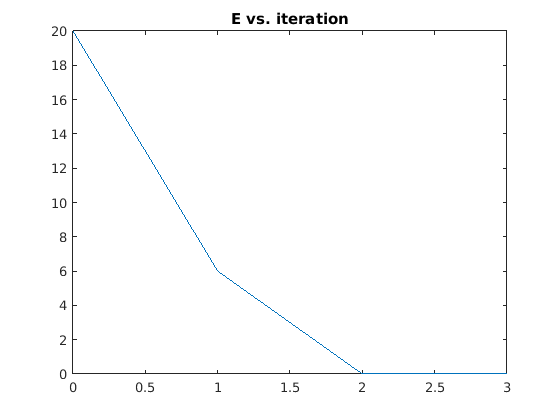
\includegraphics[width=0.75\linewidth]{E-vs-iteration}
	\caption{Minimum value of cost function after each iteration}
	\label{fig:error}
\end{figure}

\begin{figure}
	\centering
	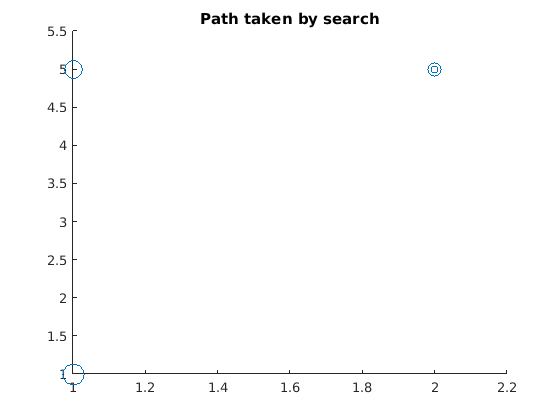
\includegraphics[width=0.75\linewidth]{path-taken-by-search}
	\caption{Path taken by the pattern search. Larger bubbles correspond to earlier approximations.}
	\label{fig:path}
\end{figure}

\subsubsection{Plot of line of fit}

A plot of the points and the line of fit can be seen in Figure \ref{fig:line-of-fit}.

\begin{figure}
	\centering
	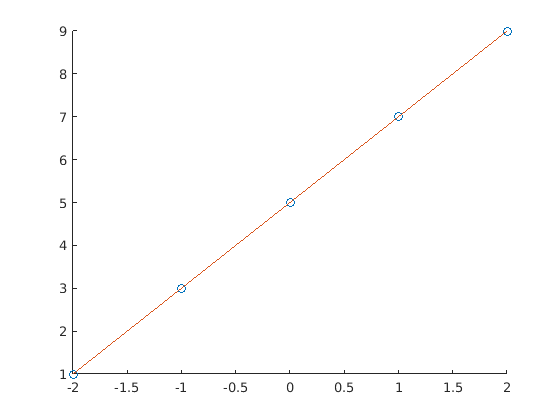
\includegraphics[width=0.75\linewidth]{line-of-fit}
	\caption{Scatter plot of points to fit and resulting line of best fit.}
	\label{fig:line-of-fit}
\end{figure}

\section{Steepest Descent}

\subsection{Objective}

A solution to the same optimization problem was approximated, but this time using the method of steepest descent.

\subsection{Formulation}

Using the method of steepest descent requires the gradient of the cost function.
The gradient of the cost function was determined analytically and is given formally as,

\begin{equation*}
E = \sum_{i=1}^{N} |y_i - ax_i - b| =  \sum_{i=1}^{N} |u_i|, \text{ where } u_i = |y_i - ax_i - b|
\end{equation*}
\begin{eqnarray*}
\frac{\partial E}{\partial a} &= \sum_{i=1}^{N} \frac{\partial u_i}{\partial a} \frac{|u_i|}{u_i} &=  \sum_{i=1}^{N} -x_i \frac{|y_i - ax_i - b|}{y_i - ax_i - b} \\
\frac{\partial E}{\partial b} &= \sum_{i=1}^{N} \frac{\partial u_i}{\partial b} \frac{|u_i|}{u_i} &=  \sum_{i=1}^{N} - \frac{|y_i - ax_i - b|}{y_i - ax_i - b} \\
\end{eqnarray*}

and $\nabla E = \begin{bmatrix} \frac{\partial E}{\partial a} & \frac{\partial E}{\partial b} \end{bmatrix}^T$.

\subsection{Source Code}

A function, \texttt{steepest\_descent}, was created in MATLAB with the purpose of minimizing the cost function.
The function takes a function handle (for the cost function), a function handle for producing the gradient of the cost function, a function handle for line searching, a tolerance at which to terminate the pattern search, a maximum number of iterations for the pattern search, a tolerance at which to terminate a given line search, a maximum number of iterations for a given line search, an initial range of search, and an initial guess at the solution.
It returns the approximate solution, the number of iterations performed, and whether or not the search converged, as output.

The source code for calculating the gradient of the cost function and searching by steepest descent are as follows.

\vspace{0.25in}
\begin{lstlisting}
function grad = lin_approx_accum_abs_error_gradient(X, a)
%LIN_APPROX_ACCUM_ABS_ERROR_GRADIENT Gradient of linear approximation cost
%
%   grad = LIN_APPROX_ACCUM_ABS_ERROR_GRADIENT(X, a)
%   Gradient of cost function that is calculated by summing absolute values
%   of differences between a linear approximation given by a(1)*x + a(2) 
%   and actual data points in two dimensions.

grad = zeros(2, 1);

rows = size(X, 1);
for i=1:rows
  error = X(i,2) - a(1)*X(i,1) - a(2);
  edir = abs(error) / error;
  grad(1) = grad(1) - X(i,1) * edir;
  grad(2) = grad(2) - edir;
end

end

\end{lstlisting}

\vspace{0.25in}

\begin{lstlisting}

function [x, iters, converged] = steepest_descent(cost_func,            ...
                                                  cost_gradient,        ...
                                                  line_search_func,     ...
                                                  steepest_descent_eps, ...
                                                  steepest_descent_iters,...
                                                  line_search_eps,      ...
                                                  line_search_iters,    ...
                                                  line_search_init_range,...
                                                  init_guess,           ...
                                                  plot_error_and_path)

if nargin < 7
  init_guess = [0; 0];
end

if nargin < 8
  plot_error_and_path = false;
end

search_range    =   line_search_init_range;
x_k             =   init_guess;
prev_cost       =   cost_func(x_k);
converged       =   false;
E(1)            =   prev_cost;
points(1,:)     =   x_k;

for iter=1:steepest_descent_iters

  d     =   -cost_gradient(x_k);
  alpha =   line_search_func(@(a) cost_func(x_k + a * d),           ...
                             search_range,                          ...
                             line_search_eps, line_search_iters);
  x_k   =   x_k + alpha * d;
  
  cost_k = cost_func(x_k);
  E(iter+1)           =   cost_k;
  points(iter+1, :)   =   x_k;
  
  if abs(prev_cost - cost_k) < steepest_descent_eps
    converged = true;
    break;
  end
  
  prev_cost           =   cost_k;
end

iters   =   iter;
x       =   x_k;

if plot_error_and_path
  plot(linspace(0, iters, iters+1), E(1:iters+1));
  title('E vs. iteration');
  figure();
  scatter(points(:,1), points(:,2), linspace(250, 25, iters+1));
  title('Path taken by search');
end

end

\end{lstlisting}

\subsection{Results}

The script \texttt{main} was appended with code to test the steepest descent algorithm.
The code added to the script and the resulting output was,

\vspace{0.25in}

\begin{lstlisting}
cost_gradient           = @(d) lin_approx_accum_abs_error_gradient(X, d);
steepest_descent_eps    = pattern_search_eps;
steepest_descent_iters  = pattern_search_iters;

tic();
[x, iters, converged]   = steepest_descent(dir_base_cf_lambda,      ...
                                           cost_gradient,           ...
                                           line_search_lambda,      ...
                                           steepest_descent_eps,    ...                                         
                                           steepest_descent_iters,  ...
                                           line_search_eps,         ...
                                           line_search_iters,       ...
                                           line_search_init_range,  ...
                                           init_guess,              ...
                                           plot_error)
toc();

\end{lstlisting}

\vspace{0.25in}

\begin{verbatim}
x =

    1.9999
    5.0000


iters =

     9


converged =

     1

Elapsed time is 0.057958 seconds.

\end{verbatim}

\vspace{0.25in}

\subsubsection{Plot the value of E at each iteration}

Plots of E at each iteration and the approximate of the solution at each iteration can be seen in Figures \ref{fig:error-sd} and \ref{fig:path-sd}, respectively.

\begin{figure}
	\centering
	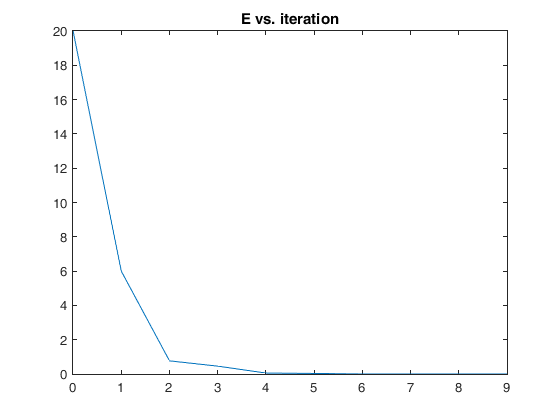
\includegraphics[width=0.75\linewidth]{E-vs-iteration-sd}
	\caption{Minimum value of cost function after each iteration for the method of steepest descent}
	\label{fig:error-sd}
\end{figure}

\begin{figure}
	\centering
	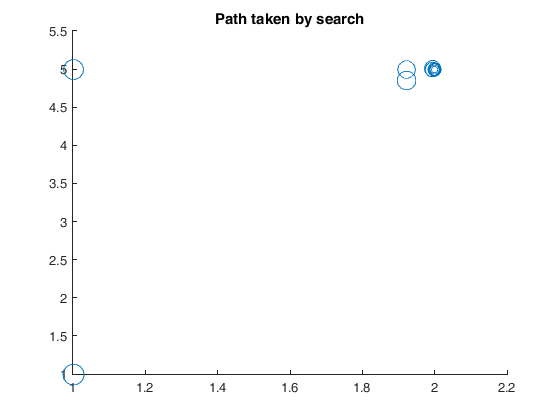
\includegraphics[width=0.75\linewidth]{path-taken-by-search-sd}
	\caption{Path taken by the method of steepest descent. Larger bubbles correspond to earlier approximations.}
	\label{fig:path-sd}
\end{figure}

\subsubsection{Comparison}

Although the method of steepest descent required more iterations, the method was faster overall (for this particular problem and on my PC's hardware).
This was probably due to the fact that the pattern search method required three line searches per iteration instead of one.
If an analytical solution to the gradient of the cost function was not available and the gradient was instead approximated numerically, this could have slowed convergence and possibly made each iteration of the method of steepest descent more costly.

\end{document}
